\documentclass[12pt]{article}
\usepackage{amsmath}
\usepackage{graphicx}
\usepackage{hyperref}
\usepackage{algorithm}
\usepackage{algpseudocode}
\graphicspath{ {./images/} }
\usepackage[a4paper, total={8in, 10in}]{geometry}
\usepackage[latin1]{inputenc}

\title{MATH4995 Project 1: Predicting Survival on the Titanic}
\author{CHOW, Hau Cheung Jasper}
\date{11 October 2021}

\begin{document}
\maketitle

\section{Introduction}
In this project, I will conduct some preliminary analysis of the Titanic dataset (available on Kaggle) and use a variety of machine learning techniques to predict which passengers survive.

\section{Data overview}
The data comes in two datasets; namely "train.csv" and "test.csv". Each row in the dataset(s) correspond to a unique passenger with a "PassengerID" identifier column and 10 features/predictors. The values of these predictors are a mix of both numerical and categorical. In the "train.csv" dataset, there is an additional column called "Survived" which contains values in the set $\{0,1\}$ describing whether that passenger survived the sinking of the Titanic (0 if they didn't, 1 if they did).\newline

\noindent train.csv dimensions: 891 x 12\newline
test.csv dimensions: 418 x 11\newline

There are a variety of ways to access the data, from downloading it directly from Kaggle via a shell command in Google Colab to having an actual copy of the file. I chose the latter approach; namely, manually, downloading the dataset from Kaggle and then uploading it to Google Drive in a designated folder where it could be easily accessed. This was because I noticed that downloading the dataset from Kaggle was necessary whenever I wanted to run the notebook, and the process took a fair amount of time.

\section{Understanding and transforming the data}
Machine learning algorithms tend to accept numerical data. As such, I had to ensure that there were no non-numerical values anywhere in the training and test datasets. I will outline the approach I used to transform the training dataset into a "machine-learning-ready" state.

\subsection{Missing values}

The first thing I did was to check which columns of the data contained missing ("NA") values. In the training dataset "train.csv", I noticed 177 missing values in "Age", 687 values missing in "Cabin", and 2 values missing in "Embarked".\newline

A brief look at the Cabin column revealed that the data tended to be in the form of "Deck-XXX" where Deck was a capital letter corresponding to which Deck that passenger was on, and XXX was some number. Since each passenger most likely occupied distinct cabins, I concluded there was no information to be gained from the specific cabin number. I did, however, extract the first letter from all data and saved it into the variable "Deck". For all missing values, I used the \texttt{fillna()} command to save their "Deck" variable as "X".\newline

In the "Embarked" section, values were one of $\{C,Q,S\}$. As such, I used \texttt{groupby()} to evaluate the median fare price for each \texttt{Pclass/Embarked} ordered pair, and filled in the missing values with the Embarked in the \texttt{Pclass/Embarked} pair whose median fare was \textbf{closest} to the fare of the missing values.\newline

In the "Age" section, there are 177 missing values out of 891 in the training set. As we can see from the distribution of the ages, if we use a more naive strategy like mean or median replacement, they are heavily centered around the middle, which is inconsistent with the original distribution.\newline

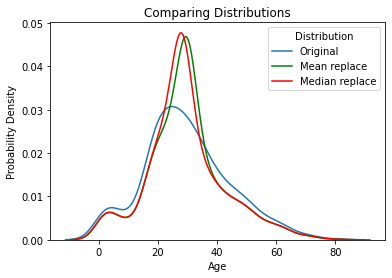
\includegraphics[scale=0.6]{age_distributions}

Therefore, we must implement a way to fill in the missing values such that the resultant distribution is at least more similar to the original. The naive way would be to compute the original distribution function, then assign 'Age' values to missing values randomly according to that distribution. However, that fails to take into account the idea that the age distribution is at least correlated with some other factors. For instance, an individual with "Mrs" in their name you would not expect to be under 18, but the naive approach would not take that into consideration.\newline

Therefore, we propose the approach of applying regression on each missing age value. Each missing Age value is defined to be the response variable $Y$ in some regression involving predictors drawn from other columns of the training dataframe, and we repeat this regression procedure until all the missing values are filled. To do this, we chose the MICE (Multivariate Imputation by Chained Equation) and a procedure called predictive mean matching (PMM) to predict a distribution and randomly select values from it to use as the missing values. This method takes into account the relations between the OTHER predictors that may be correlated with different ages, and should therefore perform better than the naive approach.\newline

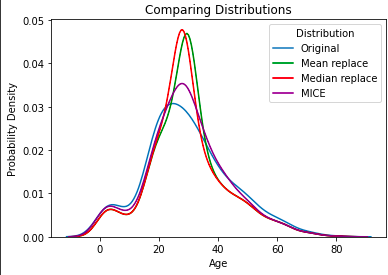
\includegraphics[scale=0.6]{mice_age_distributions}

As seen, the distribution of the MICE-fitted ages is much more consistent with the original distribution. This, of course, assumes that the missing values follow the same distribution as the ages that we do have.\newline


\subsection{Indicator columns}

We also prepared columns containing only indicator values (either 0 or 1) for the variables 'Deck' and 'Embarked'. The reason we did not leave them as a single value was because we could not safely assume that the variables were ordinal as opposed to categorical. For example, if we were to instead use a single column for a variable like 'Embarked' with values like 0 for C, 1 for Q, 2 for S might yield poor performance for any regression based model, since there is no evidence to suggest that passengers are most likely to survive if they embarked at C, then Q, then S.

\subsection{Feature engineering}

We also generated some new features from the dataset. On its own, the 'Name' column is quite useless, but after extracting the title of each individual, we were able to generate the 'Honorific' column, and then create the 'isMarried' feature (=1 for women who had the title Mrs, Ms, Mme, 0 otherwise) and the 'Unique' feature for those that had unique titles (eg Dr., Rev., Countess.)\newline

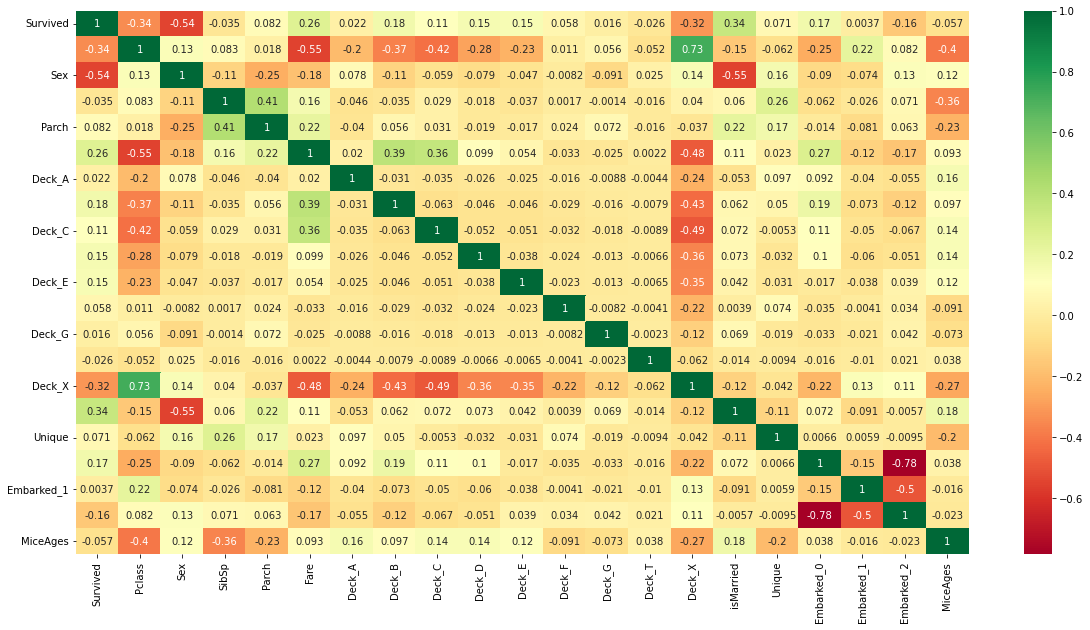
\includegraphics[scale=0.4]{corr_heatmap}

A correlation heatmap of the features show that the most important features in the model (highest absolute value of correlation) are Sex and Survived (-0.54), isMarried and Survived (0.34), Pclass and Survived (-0.34) and Fare and Survived (0.26). None of the correlations are particularly strong, but we observe a high negative correlation between values of the various indicator columns (which makes sense, since if a value is 1 in Embarked\_0, it must be 0 for all the other Embarked indicator columns.) Surprisingly, we also observe that there is a strong positive correlation between Deck\_X and Pclass (0.73) which is slightly reflected in the correlation between Deck\_X and Survived (-0.32). However, we cannot be assured of the reliability of Deck\_X as a predictor since Deck\_X denoted the missing values which made up a large proportion of the dataset.

\subsection{Visualisation}

We plotted the number of individuals that survived by gender and noticed that females over the age of 20 are disproportionately more likely to survive than males of the same age range. However, males and females under the age of 20 are approximately equally likely to survive (likely on account of them being children.)\newline

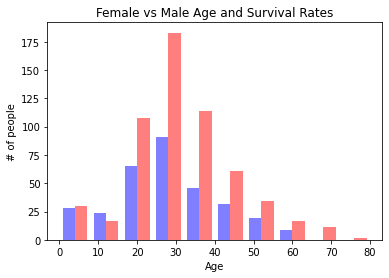
\includegraphics[scale=0.6]{female_v_male_age}

We also plotted the number of survivals by Sex, Age, Pclass, SibSp, Parch, isMarried and Unique.\newline

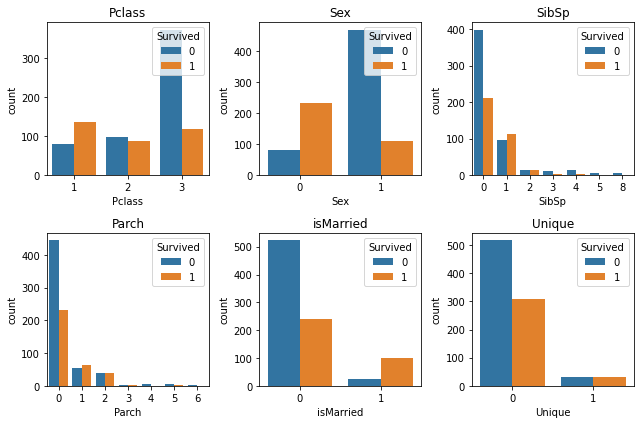
\includegraphics[scale=0.4]{factors_v_survival}

Additionally, the ratio of individuals that survived to those that didn't is the highest for Pclass=1, for married women, and for individuals with unique honorifics. Additionally, those that had one or more sibling/spouse/parent/child were also relatively likely to survive compared to if they didn't. From these visualisations, we learn more about the inherent structure of the data and can use it to do sanity checks on our model (if our predictive model underweights the importance of 'Sex', for example, clearly something is wrong).\newline

Since there is also a high correlation (0.73) between PClass and Deck\_X, to avoid collinearity, we should remove one of these features. Since Deck\_X has a high negative correlation with the other Deck indicator columns, if we removed it, we would still be able to identify a passenger from Deck\_X because all the other Deck indicator columns would have value 0 (so we are not losing any information.) Hence we shall remove Deck\_X from both the training and test dataframes. (We will also do the same for Embarked\_2 to reduce collinearity.)\newline

Therefore it makes sense to include the features 'Sex', 'isMarried', and either 'Pclass' or 'Fare' in our model.

\section{Algorithms}

We tried various approaches for determining an optimal classification. The models we tried were: k-Nearest Neighbours, Logistic Regression and Random Forest. We ignore single Decision Trees since they are susceptible to changes in training data and may tend to overfit; a random forest approach offers all the same advantages but also reduces variance.\newline

\subsection{KNN}
Our initial training accuracy of the KNN model was 0.945, which initially seems extremely good. However, this heavily implies that the k-NN model overfits to the training data, because when K=1 the probability of one sample is estimated ONLY on ONE OTHER sample, which by definition is very susceptible to noise, outliers, etc. As such we cannot assume this model's training accuracy to be indicative of its performance on the unknown test set. In fact, one common estimate of an 'optimal' value of K in a dataset with n points (in our case $n=891$ so $\sqrt{n}=29$.)\newline

When we observe the training accuracy score of the K-NN model at high values of K (23-29) we notice the accuracy score hovers around ~75\%. The validation accuracy score is around 70.9\% for the chosen value of K=29, which is slightly lower than the training accuracy score (as expected, since all models will overfit to the training dataset to a small extent.)\newline

\subsection{Logistic regression}

In logistic regression, we once again used 10-fold cross validation to estimate the test error, and the average validation training accuracy of the model (using the L2-norm and all features) was 0.8249, which was a significant improvement on KNN.\newline

\subsection{Random forest}

The 10-fold cross validation accuracy score for our random forest model with 150 estimators and maximum depth of 7 was 0.835, which was a slight improvement on logistic regression. We chose maximum depth of 7 because trees that were too deep would be overfitted to the training data, and we want our trees to be 'not collinear' with other trees. However, we admit in the 'Future Analysis' section that more work could be done in tuning hyperparameters.\newline

From our 3 models: K-NN, Logistic Regression and Random Forest, it appears Random Forest has the best training accuracy score, and even has a higher mean 10-fold cross-validation score than both the K-NN and Logistic Regression models. As such, we attempt to further tune the Random Forest model.\newline

We also chose not to use the F1-score or precision/recall metrics because those tend to be used when there is significant class imbalance (there is only a 2:1 survived:not survived ratio) AND there is greater importance in predicting one particular class over another.\newline

We further tuned our random forest model by selecting certain predictors to drop. We implement a form of backward subset selection by listing out and gradually dropping features in the random forest model starting with the least important ones. After iterating through all the features with $<0.05$ importance, we find the highest mean 10-fold CV score and compute the range of values within 1SD of that value. We notice that all of the subsets here fall within this 1SD range of values, but there is a fairly significant drop off in mean cross validation score between keeping the last feature ('Parch') and removing it, so we decide to keep the 2nd last model generated, i.e. drop all features in the list except 'Parch'. This gives our model a 10-fold mean CV score of 0.835, which is very similar compared to the original model but has the advantage of not overfitting to the least relevant features.\newline

\subsection{Future analysis}
When submitting our tuned random forest model to Kaggle, we find our test accuracy was only approximately 71\%. As such, there is clearly much room for improvement.\newline

For one, although we previously mentioned our reason for generating indicator columns, we could come up with different encodings for them (eg create a new feature called 'KnownCabin' =1 if the individual's cabin/deck number is known, and 0 if it is a missing value.) This is because may be bias that caused information about certain individuals' cabins to not be collected. This idea of using different 'encodings' of categorical variables can be extended. For instance, we can create separate features for Sibling and Spouse so that SibSp becomes two features, etc. Furthermore, we could also have attempted alternative data imputation methods besides MICE for the missing age values, since there is no guarantee that the missing age data follows the same distribution of ages that we already have.\newline

Secondly, we could experience with different metrics. In logistic regression, we could attempt to use L1 norm (which penalizes more complex models compared to using L2 norm) to prevent overfitting. Additionally, we could have also experimented with the backwards subset selection in the logistic regression model to find the optimal set of features to apply the model to instead of applying it on all of the features like we did. For validation of these models, we could also use hypothesis testing (F-test) of various logistic regression models against each other.\newline

Thirdly, we could have experimented with tuning the hyperparameters of the random forest. For instance, we could have implemented a grid search procedure for the number of estimators and the tree depth to exhaustively test various combinations, since the computational cost of the runtime is not high, this is a feasible approach.\newline

As a starting point, we observe that our 10-fold CV mean error of 0.835 is significantly higher than the test accuracy of 0.719. As such, that suggests that our original choice of parameters is already significantly overfitting to the dataset and we should choose a smaller tree depth or change the number of estimators.\newline

Finally, we could have experimented with an alternative bagging approach besides random forest; namely boosting (eg AdaBoost.) This would more heavily penalize misclassified datapoints since the loss function for boosting algorithms is exponential. However, it may have a tendency to overfit to the training data.

\section{Further fine-tuning}

\subsection{AdaBoost}

I implemented grid search for hyperparameters on AdaBoost with DecisionTree (maximum depth of 1) as base classifier. The hyperparameters I tested were \texttt{learning\_rates=\{0.01, 0.1, 0.2, 0.4, 0.7, 1, 1.4, 1.7\}} and \texttt{n\_estimators=\{10, 20, 30, 40, 50\}}. WHen the learning rates were well above 1 (eg 1.7), I noticed the training accuracy started to decrease to around 0.6, suggesting that high learning rates may lead to skipping over locally optimal solutions.\newline

 A search of the hyperparameter space revealed that the hyperparameter set specifying the simplest model within 1SD of the maximum 10-fold mean CV score was \textbf{learning rate of 0.7 and number of estimators = 10}. I also noticed that a higher number of estimators corresponded to a slightly higher 10-fold mean CV score - I will demonstrate how this is misleading later on. On the full set of predictors, this model had 0.71 accuracy on the test set, slightly lower than our original random forest result.\newline

I also tried adding backwards subset selection in conjunction with hyperparameter grid search to see if accuracy could be improved, but found that the simplified model seemed to perform even more poorly, with a test accuracy of 59.33\%, suggesting that in a boosting model, the features which the random forest deemed as irrelevant may have actually been relevant. This is quite important since the base model for my AdaBoost was a decision tree with a maximum depth of 1 and excluding many features would likely cause it to perform much more poorly, especially given that the irrelevant features were only unnecessary in a random forest model because a random forest model would have sufficient depth.\newline

To counteract the lack of features, I attempted to use the full set of predictors in Adaboost with the highest 10-fold mean CV score, namely with \texttt{learning rate=0.7} and \texttt{n\_estimators=50}, but only got a test accuracy of 40\%. Something to be learned from this is that good mean CV score is not necessarily indicative of good test performance since this model essentially has 50 estimators stacked on top of one another. Indeed, this matches with the conclusion in the lecture notes that an overly large M (number of estimators) can lead to overfitting of the training data and hence suboptimal performance on the test set.\newline

\subsection{Refining logistic regression}

Returning to our logistic regression model, I evaluated my baseline model in Part (4.2) with full set of predictors and found it does surprisingly well, with 72.01\% accuracy on the test set, and is marginally better than the original random forest model.\newline

I then considered if it would be possible to try and simplify the logistic regression model to prevent the model from overfitting on irrelevant features and avoid collinearity, just like in the random forest case. This was done by calculating the variance inflation factor (VIF), which is defined as: $VIF_{i}=\dfrac{1}{1-R^{2}(X_i)}$ where $R^{2}(X_i)$ denotes the multiple $R^2$ of predictor $X_i$ against all other predictors (i.e. the proportion of variability of predictor $X_i$ that could be explained by the other predictors.)\newline

The most common threshold indicating multicollinearity is if any one of the VIFs is $VIF_{i}>10$.\newline

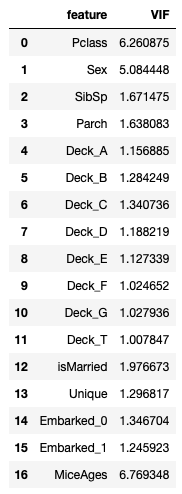
\includegraphics[scale=0.4]{vif}

In this case, none of the VIFs of the predictors satisfy this condition.\newline

To double-check the correctness of using VIF, I ended up using backwards subset selection again and found that removing predictors does seem to have a statistically significant effect on the model, since the test accuracy is reduced to 63\%.\newline

As such, there is not much to be done to improve logistic regression model either short of redesigning the features or perhaps transforming some existing features to accept quadratic terms, or perhaps including interaction terms.\newline

\subsection{Refining random forest}

I conducted hyperparameter grid search on the baseline random forest model, by generally using shallower trees so as to avoid overfitting and trees being too collinear with each other. The model with the best 10-fold mean CV score was with \texttt{n\_estimators=60} and \texttt{max\_depth=5}, but I ended up choosing the simplest model with \texttt{n\_estimators=30} and \texttt{max\_depth=5}. Test accuracy of this model was 68\%, a slight drop off. As such, this indicated that the maximum depth parameter in random forests tends to be extremely sensitive towards data. As such, I opted to select another model whose 10-fold mean CV score was within 1SD of the maximum with \texttt{n\_estimators=150} and \texttt{max\_depth=2}. This ended up performing well on the test set with accuracy of 77\%, a significant improvement over the baseline.\newline

Indeed, if the max depth is too high, then the model is extremely prone to overfitting and performing poorly on the test set. Furthermore, it is worth noting the training accuracy seems to improve as the number of estimators increases; that is to say, the amount of overfitting does NOT increase with more trees, only when the trees are deeper.

However, if analysis were to continue, additional feature engineering could be employed. Perhaps the \texttt{Name} category could be used to detect husband-wife pairs with the same last name and make the \texttt{isMarried} category include both married men and women, although this would leave out spouses who chose to travel alone or those men whose wives did not take their husband’s name. Also, the title "Master" actually used to refer to young boys or young men, and as we have seen individuals under the age of 18 tend to have higher chances of survival in both genders, so this is very likely to be a relevant feature. Finally, we could separate \texttt{SibSp} and \texttt{ParCh} into features Sibling, Spouse, Parent, Child to see if there is additional correlation (those that had parents travelling them were likely children and hence more likely to survive.)\newline

Other forms of subset selection of predictors could be used, like backward-forward elimination.\newline

Finally, I decided not to use the F1 score as a metric because that should only be used where there is significant class imbalance (there is only a 2:1 ratio in this dataset) and true positive detection of one class is much more important than false negatives of the other class.\newline

\subsection{Final performance}

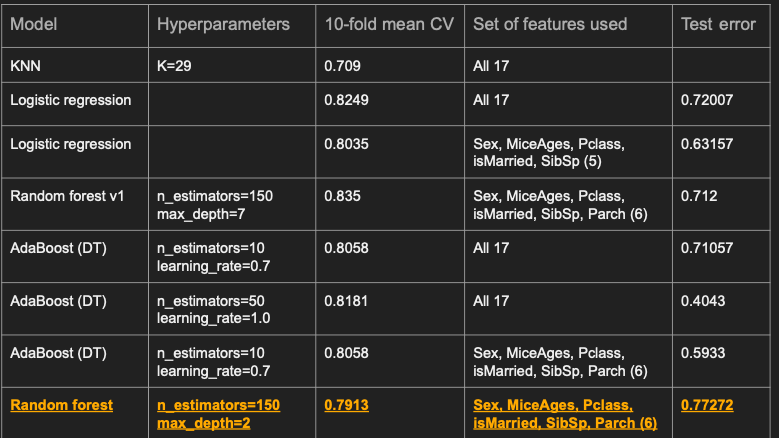
\includegraphics[scale=0.4]{final_performance}

\end{document}